\subsection{Coverage is a staircase, not a curve}
\label{sec:staircase}

A query is translatable only when \emph{every} feature it uses is supported, so for a
translator supporting exactly the feature set $S$, the share of queries all of whose
features lie in $S$ is an upper bound on $\kappa$. Choosing $S$ greedily --- at each step
the feature that completes the most queries outright --- gives an attainable set at each
size, hence a lower bound on the best ceiling a fragment of that size could reach.
Table~\ref{tab:implementation-order} is that order for Datadog and
Figure~\ref{fig:cumulative-coverage} both curves.

\begin{table}[htbp]\centering\scriptsize
\begin{tabular}{@{}rllrrr@{}}
\toprule
Step & Feature & Construct & Pending uses & Queries completed & Cumulative \\
\midrule
1 & \texttt{GROUP\_BY} & group by \{...\} & 4,922 & 20 & 1\% \\
2 & \texttt{MULTI\_QUERY} & comma-separated list of queries & 117 & 9 & 1\% \\
3 & \texttt{ARITH} & arithmetic between operands & 115 & 5 & 2\% \\
4 & \texttt{CONST} & numeric literal & 470 & 9 & 2\% \\
5 & \texttt{FUNC\_APPLIED} & function applied to the query & 205 & 1 & 2\% \\
6 & \texttt{AGG\_AVG} & space aggregator avg: & 3,885 & 1 & 2\% \\
7 & \texttt{SCOPE\_VAR} & dashboard template variable in the scope & 7,624 & 2,468 & 30\% \\
8 & \texttt{AGG\_SUM} & space aggregator sum: & 4,314 & 1,708 & 49\% \\
9 & \texttt{M\_AS\_COUNT} & .as\_count() & 1,644 & 1,079 & 62\% \\
10 & \texttt{SCOPE\_EQ} & scope term key:value & 1,347 & 974 & 73\% \\
11 & \texttt{SCOPE\_ALL} & scope \{*\} & 898 & 810 & 82\% \\
12 & \texttt{AGG\_MAX} & space aggregator max: & 275 & 245 & 85\% \\
13 & \texttt{M\_AS\_RATE} & .as\_rate() & 266 & 224 & 87\% \\
14 & \texttt{STR\_SINGLE\_QUOTED} & single-quoted string literal & 139 & 136 & 89\% \\
15 & \texttt{M\_FILL} & .fill(...) & 185 & 94 & 90\% \\
16 & \texttt{SCOPE\_GLOB} & wildcard in a scope value & 143 & 89 & 91\% \\
17 & \texttt{SCOPE\_NEG} & negated scope term !key:value & 134 & 91 & 92\% \\
18 & \texttt{M\_WEIGHTED} & .weighted() & 70 & 64 & 93\% \\
19 & \texttt{AGG\_COUNT} & space aggregator count: & 58 & 53 & 93\% \\
20 & \texttt{SCOPE\_BOOL} & boolean scope (AND / OR / NOT) & 160 & 37 & 94\% \\
\bottomrule
\end{tabular}

\caption{Greedy implementation order for Datadog. ``Pending uses'' is how many queries
still need the feature when it is chosen; ``queries completed'' how many it finishes on
its own. The cumulative column bounds $\kappa$ for a translator limited to those
features.}
\label{tab:implementation-order}
\end{table}

\begin{figure}[htbp]\centering
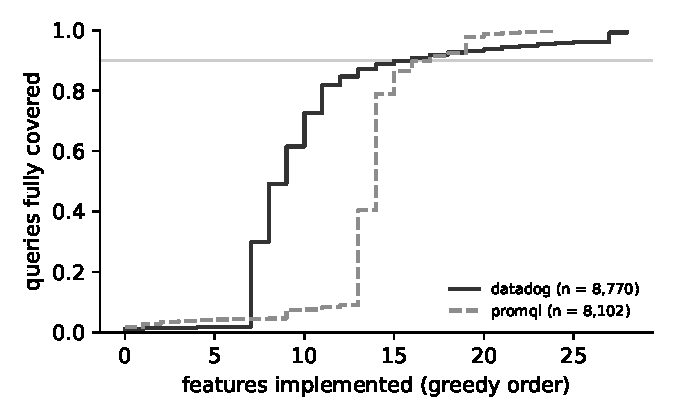
\includegraphics[width=0.62\linewidth]{figures/cumulative_coverage}
\caption{Queries fully covered against features implemented, in greedy order. The line
at $0.9$ marks the level reached after sixteen of Datadog's twenty-eight features and
seventeen of PromQL's twenty-four.}
\label{fig:cumulative-coverage}
\end{figure}

The shape is the finding. The first six Datadog features complete $45$ queries between
them --- $0.5\%$ of the corpus, on top of the $1.1\%$ that use no feature at all --- and
then template-variable scopes and \texttt{sum:} take two steps to $49.2\%$. Half the corpus
needs nine features; $90\%$ needs sixteen of the twenty-eight. PromQL behaves the same way
and slightly worse: its first six features complete $221$ of $8{,}102$ queries
($2.7\%$), half the corpus needs fourteen features and $90\%$ needs seventeen of
twenty-four.

For anyone building one of these translators this is the practical result of the paper. A
partial translator is worth almost nothing: there is no prefix of the feature list that
buys proportional coverage, because coverage is conjunctive over features while
popularity is marginal. The ``$80\%$ of queries with $20\%$ of the work'' intuition is
simply false here, and that asymmetry is a switching cost in its own right --- an
incremental migration cannot show incremental progress.

